\documentclass[12pt ,a4paper ]{article}

\usepackage[utf8]{inputenc}
\usepackage[T1]{fontenc}      % caractères français
\usepackage[french]{babel}  %langue
\usepackage[left=2.3cm,right=2.5cm,bottom=2.5cm,top=2.3cm]{geometry}   % marges
\usepackage{verbatim}
\usepackage{float}
\usepackage{graphicx}         % images
\usepackage{verbatim}
\usepackage{multicol}
\usepackage{titlesec}

\usepackage{hyperref}
\usepackage{url}
\usepackage[hyphenbreaks]{breakurl}
\hypersetup{
    colorlinks=true,
    linkcolor=blue,
    urlcolor=blue,
}

\urlstyle{same}


                           
\begin{document}
	\begin{titlepage}
		
		\vspace{0.5cm}
		\begin{center}		
			{\Large  Master 1 Informatique}
		\end{center}
		\vspace{1cm}
		
		\rule{1\linewidth}{1.1pt}\newline   %regle
		\begin{center}
			 {\Huge \textbf{Rapport de Projet : Traitement Automatique du Texte en IA}}
		\end{center}
		\rule{1\linewidth}{1.1pt} \\
		
		\begin{center}
		\begin{LARGE}
		\textbf{Sujet :} \\\vspace{0.6cm} Identification des opinions exprimées dans les avis et commentaires d’un ordinateur.
		\end{LARGE}
		\end{center}
		
		\vspace{0.5cm}
		\begin{center}	
				\begin{Large}
				Yann MARTIN D'ESCRIENNE \\ 
				Yohann TOGNETTI \\ 
				\end{Large}
		\end{center}
		\vspace{6cm}
		
		\begin{center}
			{\large « Année universitaire 2020 - 2021 »}
		\end{center}
		

\end{titlepage}

\newpage
\tableofcontents 
				
\newpage


\begin{multicols}{2} 
\section{Introduction}

	\subsection{Présentation générale du projet}
		Dans le cadre de notre cours de Traitement automatique du texte en IA, il nous a été demandé d'effectuer un projet de notre choix impliquant une intelligence artificielle travaillant sur des données textuelles. La restriction sur le sujet se limitant à l'existence d'un jeu de données conséquent.
	
	\subsection{Choix du sujet}
		Notre choix de sujet fut \textbf{l'identification des opinions exprimées dans les avis et commentaires d’un ordinateur.} Plus précisément, comment retrouver parmi un ensemble de commentaires les parties de l'ordinateur visées,  sur quels aspects et quel en est l'avis général qui en ressort. 
		
\section{Description des tâches}
Ce sujet est fortement inspiré du « SemEval-2015 Task 12 » sur la partie « Aspect Based Sentiment Analysis (ABSA): Laptop Reviews » et partage donc le même objectifs avec des simplifications. Les différentes entités et catégories qui vont suivre provienne également des annotations du sujet de SemEval. Chacun des commentaires est fragmentés phrase par phrase afin de faciliter le travail de l'IA. 
		
\subsection{Entités}
\noindent Tout d'abord il s'agit de retrouver dans la phrase le(s) entité(s) ciblée. Elles peuvent être l'ordinateur comme un tout, ses parties physique (clavier, écran..) , des logiciels ou OS (Windows, navigateur, jeux...) ou bien même une compagnie et ses services. (DELL, Apple, le support technique, la livraison..).\\

\noindent\textit{Remarque : } Rien n'interdit d'avoir plusieurs entités dans la même phrase.\\
		
\noindent Voici la liste des entités possible : 
\begin{itemize}
\item DISPLAY (=moniteur, écran), 
\item CPU (=processeur), 
\item MOTHERBOARD (=carte mère),
\item HARDDISC (=disque dur), 
\item MEMORY (=mémoire, RAM), 
\item BATTERY (=batterie), 
\item POWER\_SUPPLY (=chargeur, unité de chargement, cordon d'alimentation, (power) adapteur),
\item KEYBOARD (=touche, clavier, pavé numérique), 
\item MOUSE (=sourie, pavé tactile)
\item FANS\_COOLING (=ventilateur, système de refroidissement), 
\item OPTICAL\_DRIVES (=lecteur CD, DVD ou Blue-ray),
\item PORTS (=USB, HDMI, VGA, lecteur de carte),
\item GRAPHICS (=carte graphique, carte video),
\item MULTIMEDIA\_DEVICES (=son, audio, microphone, webcam, haut-parleur, casque, écouteurs).
\end{itemize}				

\subsection{Catégories}
\noindent Une fois obtenue il faut également trouver sur quelle(s) catégorie(s) de l'entité le commentaire porte. Cela peut être un aspect général , sa prise en main, ses performances, son design et ses fonctionnalités, etc... \\

\noindent\textit{Remarque : }Là encore, rien n'interdit d'aborder plusieurs catégorie pour la même entité au sein d'une même phrase.\\

\noindent Voici la liste des catégories possible : 
\begin{itemize}
\item GENERAL, 
\item PRICE (=prix), 
\item QUALITY (=qualité), 
\item DESIGN\_FEATURES (=design et fonctionnalités),
\item OPERATION\_PERFORMANCE, 
\item USABILITY (=ergonomie, prise en main), 
\item PORTABILITY (=portabilité),
\item CONNECTIVITY (=connectivité), 
\item MISCELLANEOUS (=divers).
\end{itemize}	

\paragraph{} 
\noindent L'entité E et la catégorie C qui s'y rapporte forme ainsi un couple E\#C. \\

\noindent\textit{Remarque : }Il est à noter la possibilité qu'aucun couple E\#C ne se rapporte à une phrase d'un commentaire. Nous ne relevons pas l'état \textit{OUT OF SCOPE} comme dans le SemEval, quand elle a raison, notre IA ne répondra juste rien. 

\subsection{Polarité}
Enfin, chaque phrase (et non chaque couple E\#C comme dans le sujet de SemEval) se verra attribuer une polarité. Les valeurs de cette polarité sont : \textbf{negative} pour les phrases soulignant des défauts ou de mauvais avis, \textbf{positive} pour celles qui au contraire mettent en valeur des points ou des avis positif, \textbf{neutral} lorsque la phrase ne met pas d'opinion en avant et donne par exemple un conseil et finalement \textbf{mixed} pour les textes critiquant un aspect de l'ordinateur mais appréciant un autre. 

\section{Jeux de données}
Les jeux de données se divisent en deux groupes : le jeu de données d'entrée correspondant à ce que l'IA va utiliser pour s'entrainer et celui de test sur lequel les mesures seront effectuées. Tout deux proviennent du site du SemEval. 

\subsection{Structure des jeux de données}
\noindent Ce sont tout deux des documents XML possédant la structure suivante (simplifiée) :  

\begin{figure}[H]
\begin{center}
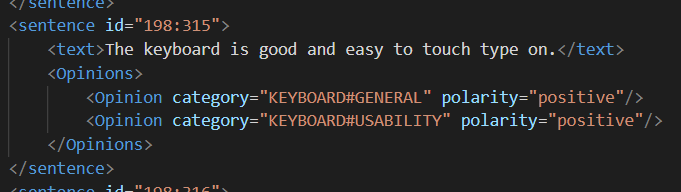
\includegraphics[scale=0.55]{xml_struct.png}
\caption{\small{structure du fichier XML}}
\end{center}
\end{figure}

\subsection{Modification des jeux de données}
Suite à notre implémentation de notre IA qui sera décrite dans le chapitre suivant, de nombreux problèmes nous ont forcés à ajouter nous même des phrases dans le jeu de données d'entrainement.\\

En effet notre IA répond de la présence ou non de chaque couple E\#C dans la phrase actuelle pour chaque combinaison d'entité E et catégorie C. Cela se traduit par une nécessité de nombreuses données appartenant à chacun des couples pouvant apparaitre afin d'obtenir une fonction d'évaluation optimale. 

\paragraph{}
\noindent Environ 350 phrases ont été ajoutées, toutes sont la section 'sentences' d'\textbf{ID 198}. Certaines proviennent d'avis de consommateur sur les ordinateur portables les plus commentés sur Amazon (en anglais), notamment pour les phrases portant sur les clavier, écran, pavé tactile et batterie. Nous avons rédigés le reste pour les catégories plus complexe et moins abordées en générale. Par exemple la qualité des lecteurs DVD ou bien l'ergonomie des OS. \\ 

\noindent \textit{Remarque : } Il est à noté que certain couple n'apparaissent ni dans les données d'entrainement, ni dans les données de test. Par simplification, ces couples ont été ignorés et aucunes phrases n'est étiquetées avec.

\begin{figure*}[ht]
    \begin{center}
        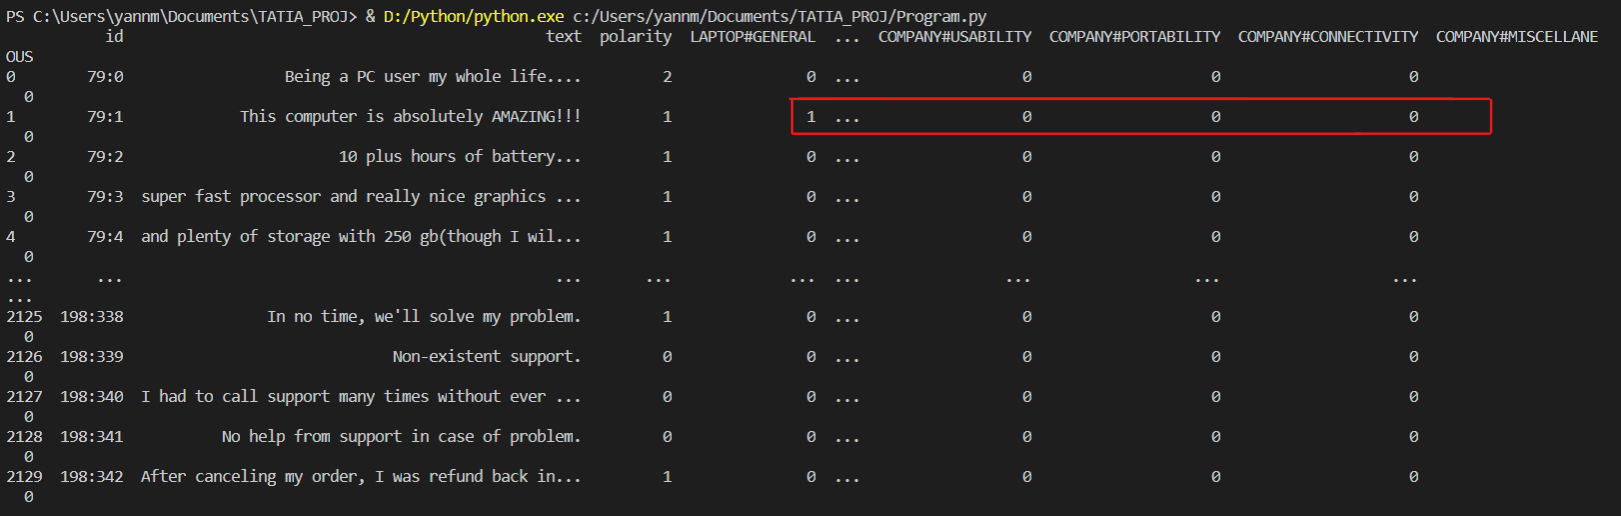
\includegraphics[width=1\textwidth]{first_dataf.png}
    \end{center}
\caption{\small{dataframe du fichier XML}}
\end{figure*}

\newpage
\section{Implémentation de l'algorithme}
Notre algorithme est développé en python. Il se divise en 4 fichiers de code ayant chacun un rôle précis dans l'implémentation de l'algorithme d'apprentissage. 

\subsection{DataInitializer.py}
Ce fichier permet de lire un documents XML du jeu de données et regroupe les informations essentielles dans un dataframe de la librairie \textit{panda}. Chacune des phrases correspondent à une ligne dans le dataframe. \\

\noindent Il vient tout d'abord récupérer l'ID et le texte de chaque phrase. \\

\noindent Ensuite il récupère chaque couple E\#C et transforme le tout en un vecteur binaire ayant des 1 uniquement aux colonnes correspondant au couple comme sur l'image ci-dessus. Étant donné le nombre de couples possible, il s'agit d'une vecteur à 197 dimensions comportant majoritairement des 0.\\

\noindent Finalement, le programme récupérera la polarité de chaque couple E\#C et en conclue une polarité générale de la phrase selon les règles suivantes :
\begin{enumerate}
\item \textbf{\small{neutral + X = X, X une polarité. }}
\item \textbf{\small{positive + negative = mixed.}}
\item \textbf{\small{mixed + X = mixed, X une polarité.}}
\end{enumerate}

\noindent Cette polarité général est ensuite convertie en entier:

\noindent \textbf{0=negative, 1=positive, 2=neutral, 3=mixed.}

\subsection{PreProcessing.py}
Ce fichier permet d'effectuer un pré traitement sur les textes du premier data frame afin de facilité le travail d'apprentissage de l'IA. Il s'appuie notamment sur la librairie \textit{nltk}.\\

\noindent Tout d'abord le texte va être mit en minuscule afin de ne pas différencier des mots n'ayant pas la même casse. Ensuite chacun de ses mots (y compris la ponctuation) va être transformé en \textbf{« token »}. De ces tokens sera retiré la ponctuation ainsi que ce que l'on appelle les \textbf{STOPWORDS}. Ce sont les mots n'ayant pas de grande valeurs syntaxique comme les déterminants, adjectifs possessifs, conjonctions de coordination, verbes communs (être, avoir)...\\

\noindent L'étape suivante consiste à effectuer une \textbf{lemmatisation} sur chacun des tokens. La lemmatisation est un traitement lexical qui consiste à appliquer aux verbes, substantifs, adjectifs... un codage renvoyant à leur entrée lexicale commune, leur « forme canonique ».\\\\

\noindent \textit{Exemple :}\\
Les / la\\
étoiles /étoile\\
claires / clair\\
luisent / luire\\
noire / noir\\

\noindent Voici une image des phrases du dataframe précédent où celles-ci ont été pré-traitées : 
\begin{figure}[H]
    \begin{center}
        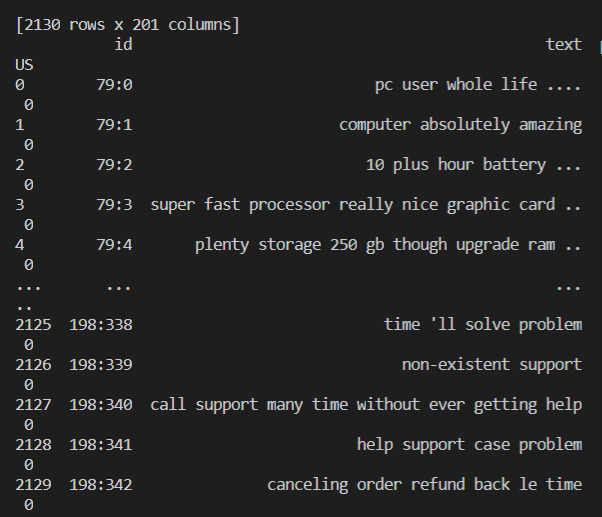
\includegraphics[scale=0.62]{pretrait_dataf.png}
    \end{center}
\caption{\small{Phrases pré-traitées}}
\end{figure}

\subsection{Classify.py}
Ce fichier a pour fonction de créer un classificateur pour chaque classe qui possèdent des données pour s'entrainer. L'intégralité de ce fichier utilise principalement la librairie \textit{sklearn} qui est une librairie complète pour l'apprentissage d'une IA.\\

\noindent \textit{Remarque : } 
Certaine classe n'étant pas existante dans les données d'entrainement, elle n'ont donc pas de classificateur attitré.\\

La première opération à faire pour pouvoir créer un classificateur, est de transformer les phrases en vecteurs. Pour cela, nous avons utilisé \textbf{TfidfVectorizer} de la librairie sklearn. Au niveau des paramètres, nous avons décidé d'utiliser la norme "l2" et d'utiliser des ngram entre 1 et 8. Une fois créée nous avons entrainé ce vectoriseur avec les commentaires de notre jeu de d'entrainement.\\

Ensuite, nous pouvons commencer la classification. Pour celle-ci nous avons décidé d'utiliser la méthode one-versus-rest (« une contre le reste »). Cette méthode consiste à traiter chaque classe indépendamment des autre. Chaque classe représente ici un de nos couple E\#C.\\

Dû au peu de données présente pour certaine classe, et l'effort pour en ajouter d'autre étant trop élevé, nous avons eu recourt à un algorithme d'échantillonnage pour augmenter les classes minoritaires. Cet algorithme n'est autre que \textbf{ADASYN} (Adaptive Synthetic). A partir des données existantes (au moins 5 ici), l'algorithme va en créer d'autre en utilisant le principe des « K plus proche voisins ». L'image ci-dessous montre l'efficacité d'ADASYN.\\

\begin{figure}[H]
    \begin{center}
        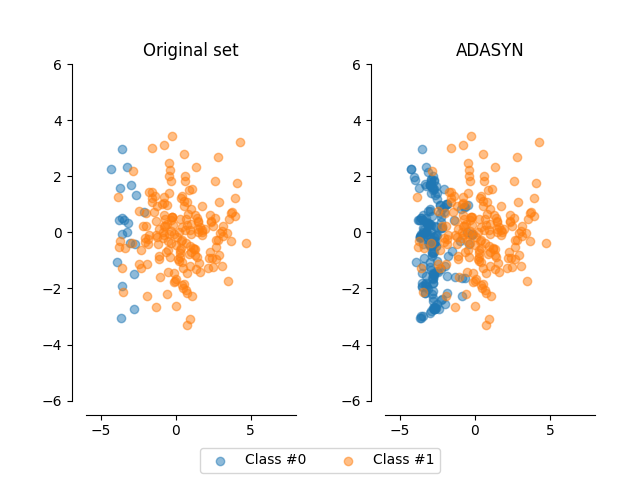
\includegraphics[scale=0.62]{adasyn.png}
    \end{center}
\caption{\small{L'algorithme ADASYN}}
\end{figure}

Après avoir fait cela, il nous reste plus qu'a entrainer chacun des classificateur. Nous avons utiliser donc utilisé \textbf{OneVsRestClassifier} avec comme solver "sag", un poids equilibré entre chaque classe et un nombre d'itération maximum de 1000. Afin de pouvoir réutiliser ces classificateurs pour notamment évaluer une phrase à la volée, nous les stockons dans un dictionnaire ayant pour clé la catégorie et pour valeur le classificateur.\\

La dernière fonction de cette classe est la prédiction un dataframe test. Pour ce faire, à l'aide du vectoriseur et des classificateur, il nous suffit de pré-traiter et vectoriser chaque phrases et d'appeler pour chacune l'intégralité des classificateurs stockés dans le dictionnaire pour prédire à quelles classes (ou couple E\#C) appartient chaque commentaire.

\subsection{PlotResult.py}
Ce fichier utilise la libraire \textit{matplotlib} de python. Il permet de mettre en place la représentation graphiques des résultats obtenus. Les données sont récupérées lors de la classification du fichier précédent, puis sont misent dans des diagrammes en barre. Cela permet d'avoir une vision générale mais rapide des différents score évalués. En effet il y a beaucoup de classe différentes et un rapport de classification détaillés pour chacune d'elle ne serais pas pertinent.

\begin{figure*}[t]
    \begin{center}
        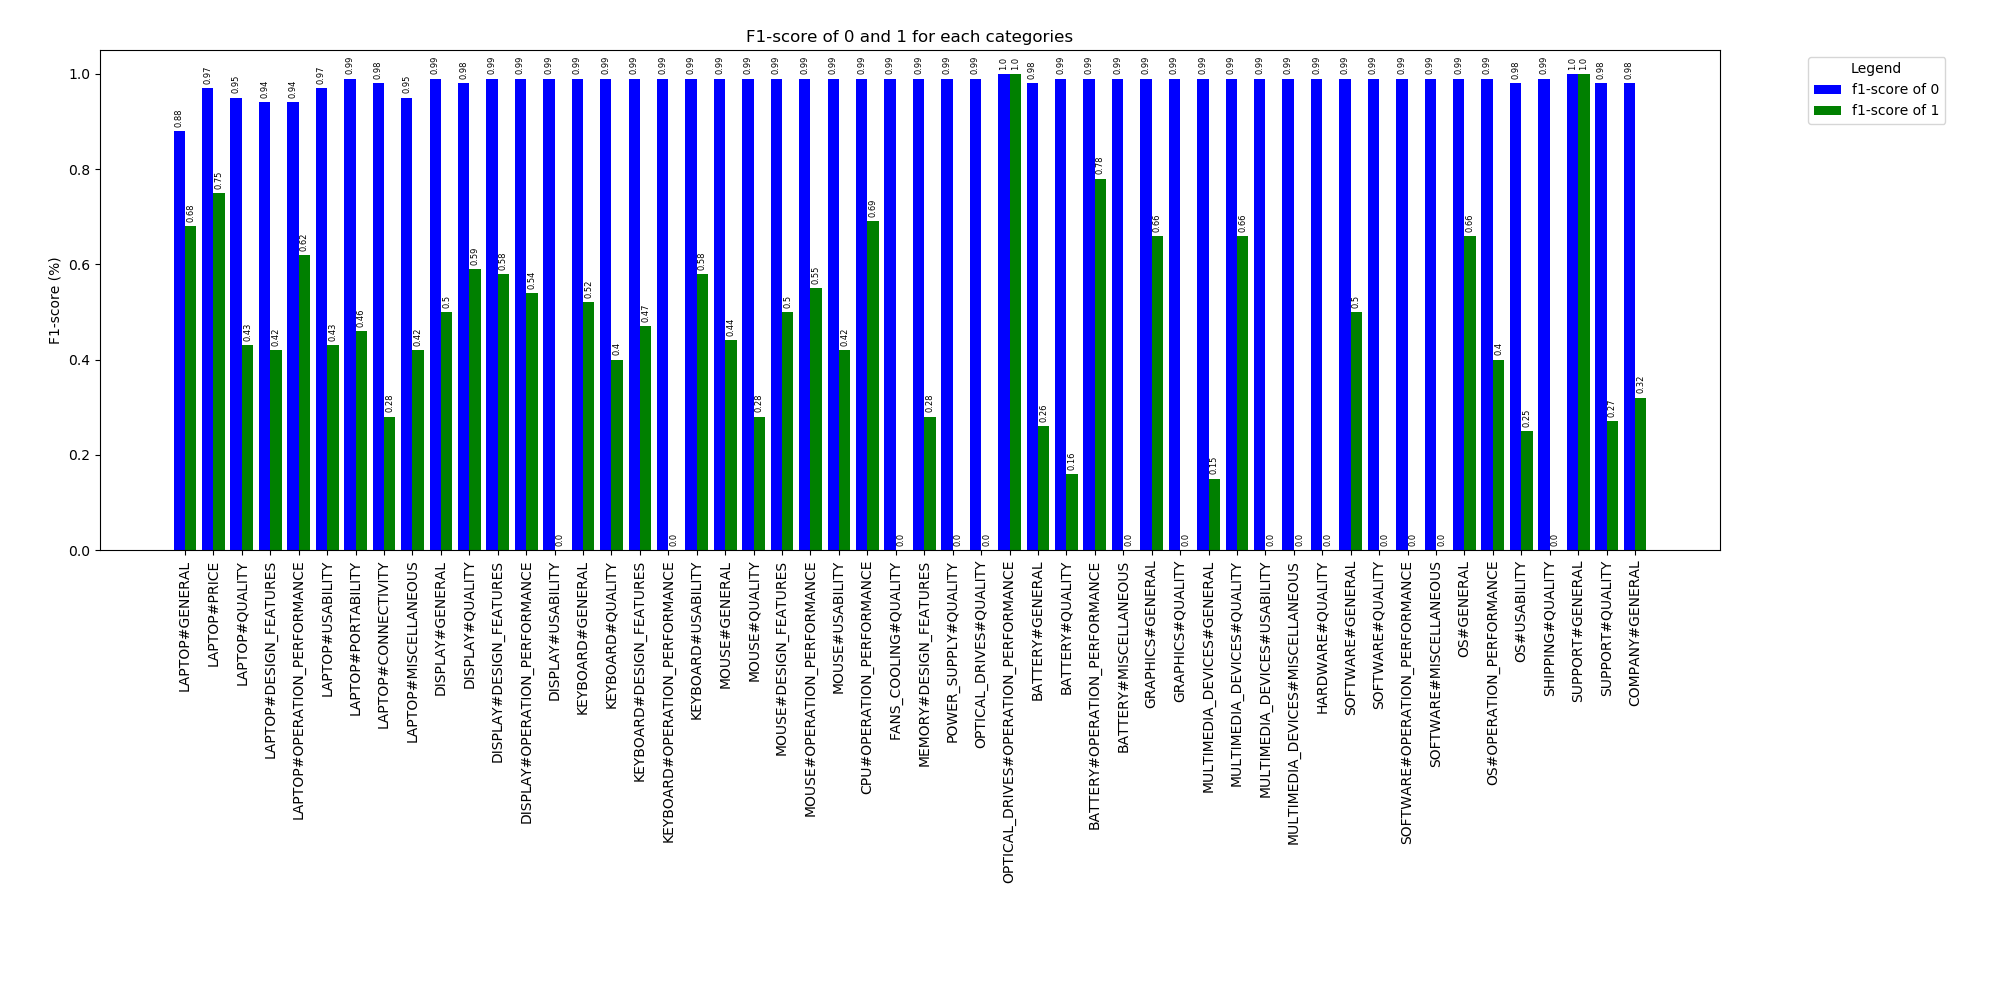
\includegraphics[width=1.15\textwidth]{data_plot.png}
    \end{center}
    \caption{F1-score de chaque classe pour 0 et 1}
\end{figure*}
\newpage
\section{Résultat obtenus}
Il est à noter que les résultats peuvent être légèrement différent à chaque appel du programme ainsi les graphiques qui vont suivre ne sont pas forcément absolus. 

\subsection{Résultat général}
Il est facilement remarquable sur la \textit{figure 5} que la valeur 0 (donc l'absence du couple E\#C) possèdent un bien meilleur score que la valeur 1. En effet un commentaire parlant d'un clavier uniquement ne vont pas parler d'un écran ou d'une souris, ce qui créer un nombre conséquent de données négative (c-à-d 0) pour chaque classes. Il est alors plus facile pour l'IA de déterminé si la phrase n'appartient pas à un couple que l'inverse.\\

On constate effectivement que le f1-score des valeurs 1 de chaque classe est assez variable et atteins parfois même 0\%. Cela s'explique avec deux raisons.
 
\noindent Soit par une précision de 0\%, car certain couple dans les données de test n'ont qu'une apparition ce qui rend le résultat binaire ou bien simplement par l'échec de l'IA à classer correctement les phrases des données de test (les justifications de cette lacune sera expliquée dans l'analyse du résultat suivant). 

\noindent Soit par un recall faible, car l'IA peut facilement trouvé la bonne entité mais pas la bonne catégorie et vis-versa, et cela se traduit par une réduction du recall et donc du f1-score.\\

Comme dit précédemment, la valeur du f1-score des valeurs 0 est très élévé, environ 95\%, ainsi ne nous y attarderont pas plus que ça et nous concentrerons plus sur les résultats et scores obtenus pour les valeurs 1.

\begin{figure*}[t]
    \begin{center}
        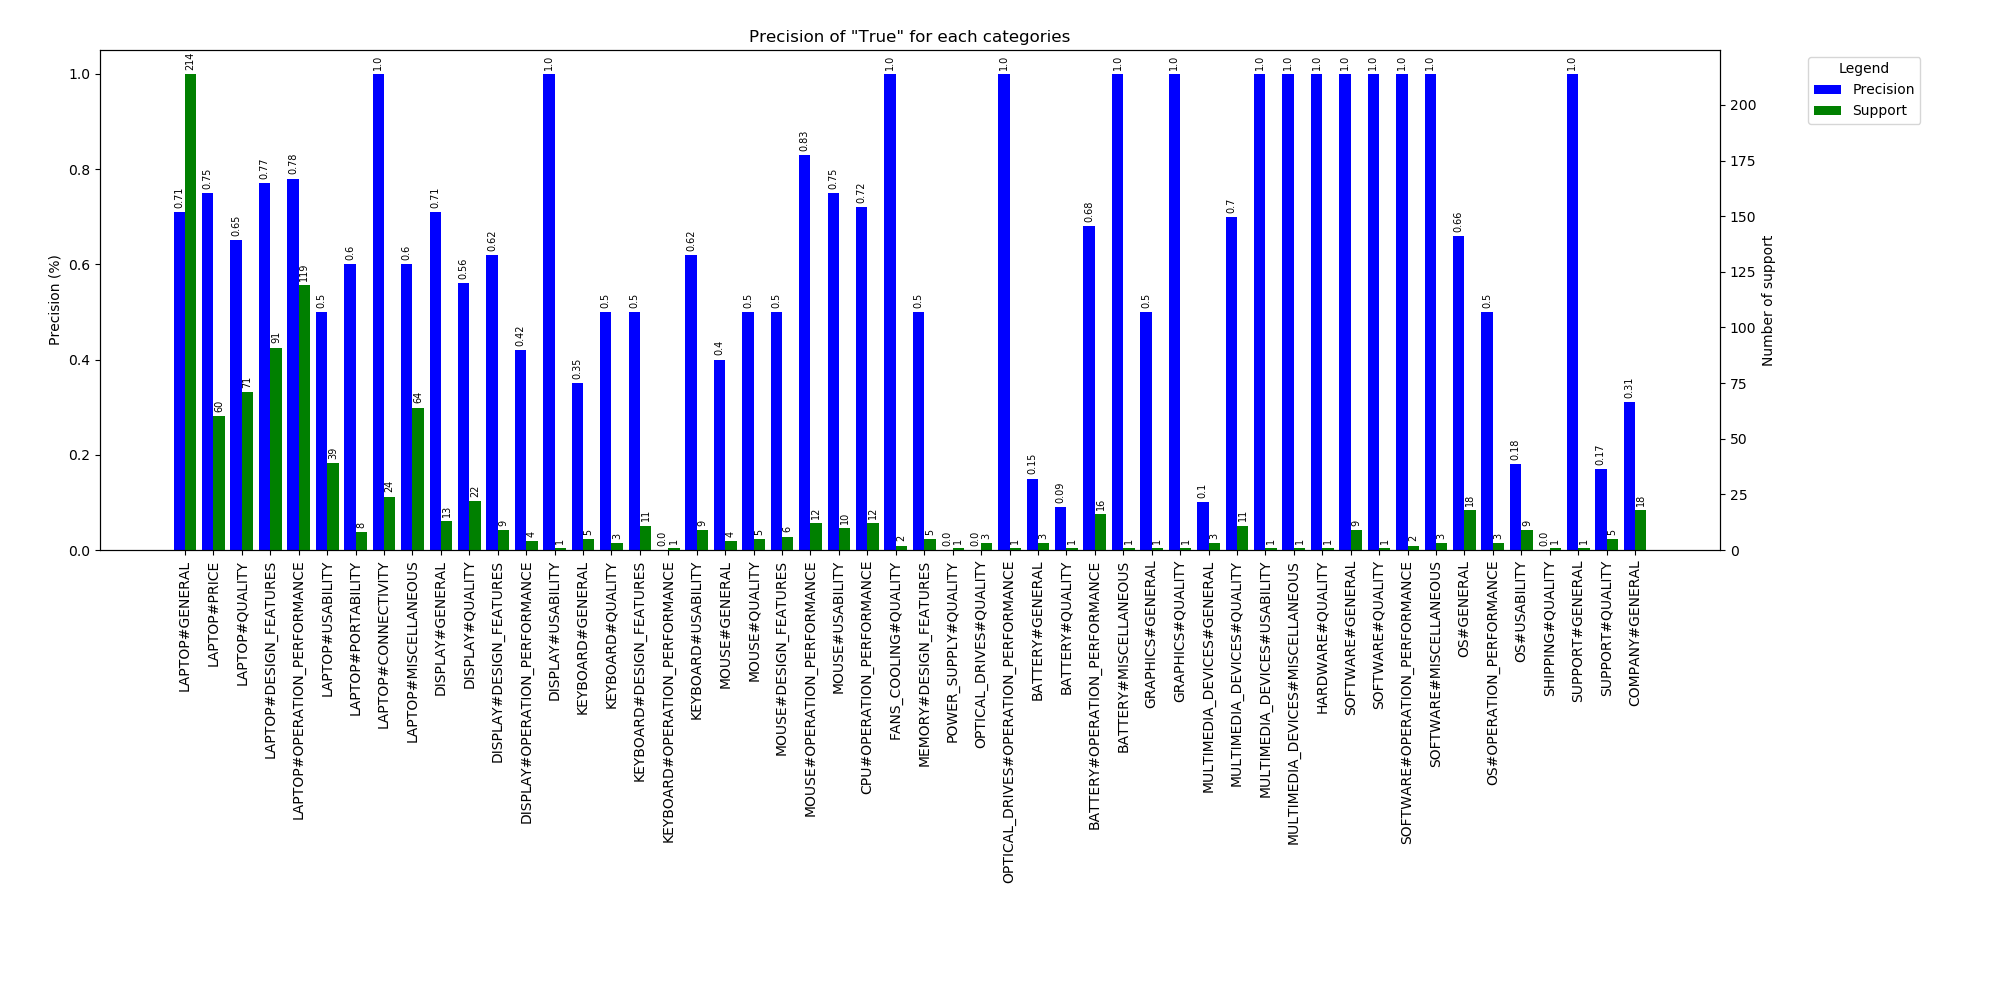
\includegraphics[width=1.15\textwidth]{true_data_plot.png}
    \end{center}
    \caption{précision et support de la valeur 1}
\end{figure*}
\newpage
\subsection{Résultat pour la valeur 1}
On remarque premièrement que les précisions de chaque couple E\#C ne sont pas homogène. Cela s'explique par la différence majeure entre chaque entités et les catégories qui s'y rapporte. En effet il est beaucoup plus simple et parler de l'ergonomie d'une souris (ou d'un pavé tactile) que de l'ergonomie d'un OS, ce qui explique l'écart de précision entre ces deux couples. \\

De plus, certain couples possèdent un jeu de données qui se veut parfois peu ressemblant entre chaque élément y appartenant. Par exemple, pour parler d'un clavier, il y aura beaucoup de chance de trouver les mots "touche","clavier" ou bien "pavé numérique", ce qui focalise l'IA sur certain éléments clés et en ressort une bonne précision. Mais par exemple, le couple \textit{COMPANY\#GENERAL} peut très bien parler de Window comme d'Apple, Dell , toshiba ... de mille et une façon, ce que l'IA a du mal à assimiler. \\

Enfin, une relation logique apparait entre le support (nombre d'éléments) et la précision. Moins on a de données plus la précision est extrême (0\% ou bien 100\%) car soit l'IA a tout juste, soit tout faux. Au contraire, lors d'une présence d'un nombre de données assez conséquent (environ 10), la précision tend à dépasser les 50\% ce qui pourrait être plus représentatif du niveau de classification de l'IA. Par exemple le nombre de données le plus élevé (214) est celui du couple \textit{LAPTOP\#GENERAL} (ce qui est assez logique en soit) et il possède une précision de 71\%.

\begin{figure*}[t]
    \begin{center}
        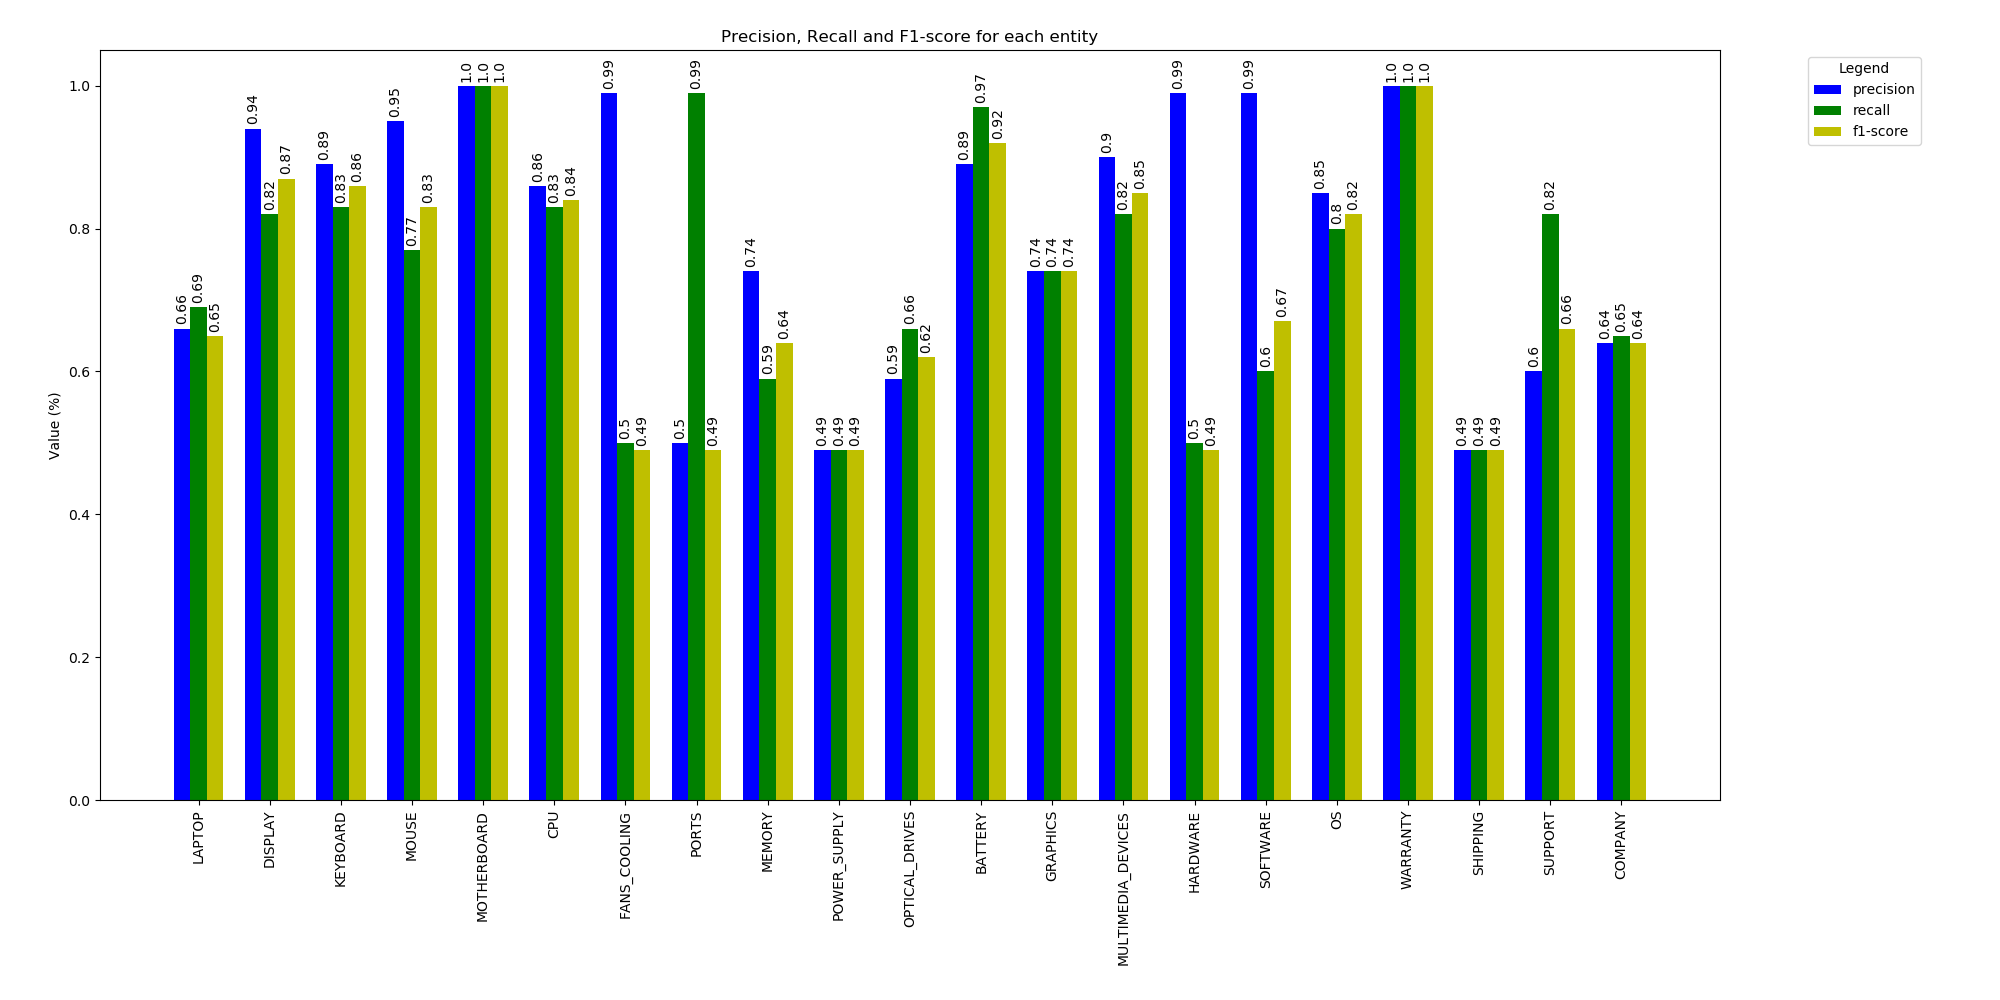
\includegraphics[width=1.15\textwidth]{entity_plot.png}
    \end{center}
    \caption{score par entités}
\end{figure*}
\newpage
\subsection{Résultat par entités}
Suite à de nombreux tests sur des classifications de phrases, nous avons remarqué que l'IA se trompe parfois dans le ou les couple E\#C mais arrive tout de même à reconnaitre la ou les entités E qui est la cible de la phrase. Nous avons donc regroupé par entité et avons calculé la precision, le recall et le f1-score de chacune.\\

Là encore attention, malgré le regroupement par entité, certaines n'ont qu'un seule données, ce qui explique les scores à 50\%. En effet nous avons récupéré la macro-moyenne et non la moyenne pondérée car celle-ci est figé à 99\% pour toutes les entités (dû à grand nombre de cas à 0 et très peu d'erreur de l'IA dessus comme expliqué précédemment), il n'est donc pas intéressant de faire une étude dessus. Cette macro-moyenne se retrouve donc à cette valeur lorsqu'il n'y a qu'une donnée pour la valeur 1 et que l'IA ne retrouve pas la bonne entité E suivant le simple calcule suivant : 

\begin{equation}
(99 + 0) / 2 \simeq 50 \%.
\end{equation}

Mis à part ces cas précis, les scores obtenus sont relativement corrects et on peut facilement affirmer que l'IA arrive à reconnaitre les entités cible d'un commentaires. Toutefois, nous avons remarqué que lorsque la phrase aborde différentes entités de manière brève, par exemple \textit{"L'ordinateur est cool, le clavier et le son sont correct mais l'affichage est magnifique"}, la classification de toutes ces entités semble très difficile pour l'IA. \\

\begin{figure*}[t]
    \begin{center}
        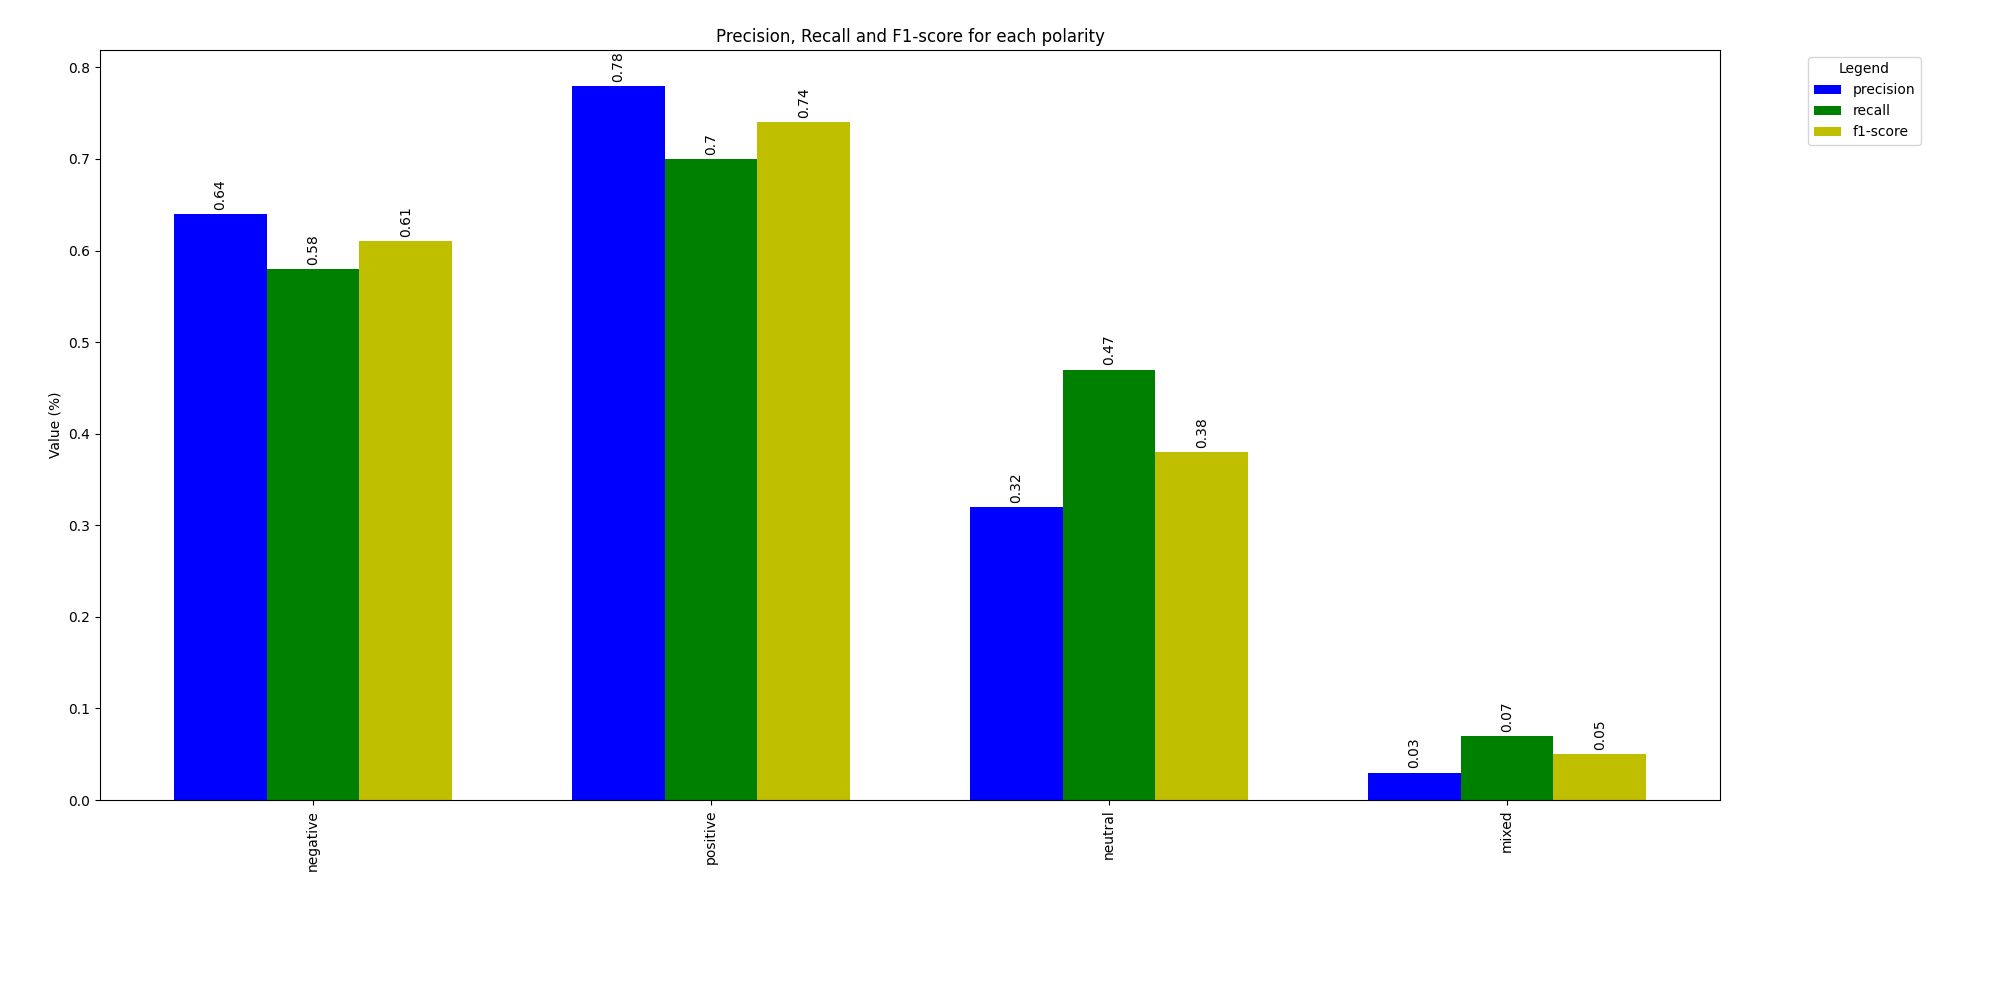
\includegraphics[width=1.15\textwidth]{polarity_plot.png}
    \end{center}
    \caption{score de la polarité}
\end{figure*}
\newpage
\subsection{Résultat de la polarité}
Tout d'abord voici le nombre de données de base par polarité :
\begin{itemize}
\item negative : 768
\item positive : 917
\item neutral : 430
\item mixed : 46
\end{itemize}
\medskip
On constate que la précision, le recall et le f1-score sont relativement proche pour chaque polarité ce qui ne souligne pas de problème particulier dans une classe. 
Il est notable que \textit{positive} et \textit{negative} sont les classes qui comportent le plus de données, il est donc normal que leur score soit les plus élevés. \\

Le fait d'avoir un commentaire positif semble d'ailleurs plus facile à détecter qu'un commentaire négatif. Cela s'explique par le fait que souvent, un commentaire négatif consiste en l'énumération des défauts de l'ordinateur sans forcément de mot clé signifiant une insatisfaction ou un mécontentement, l'IA à donc plus de mal à déterminé si cela est négatif (une énumération de fait pouvant être neutre). \\

Ainsi, la polarité neutre peut ressortir également de plusieurs tournure de phrase. Aucun mot clé n'est propre à un avis neutre, ce qui rend plus difficile sa classification et lui donne des score relativement médians. \\

Finalement, la polarité mixed possède le score le plus bas car d'une part, le jeu de données est très faible relativement aux autres, mais également, c'est la polarité la plus dure à classifié et n'existe pas réellement. Nous l'avons créer dut à la simplification que nous avons faite d'avoir une polarité générale et non propre à chaque couple E\#C. Il est donc évident qu'elle n'est pas absolue et consiste à la fusion d'un avis positif et négatif. 

\section{Les améliorations possibles}
Maintenant, nous allons voir ce que nous aurions pue améliorer a notre projet.

\subsection{Les classe}
Le plus gros problème de notre sujet sont les classes qui on était choisi pour le jeu de données, il y en a beaucoup trop (126) dont la plupart qui sont similaire. Avec plus de temps, il aurais était préférable de refaire la plupart des classe sans garder la forme entité\#categorie. Car pour des phrase de type "L'ordinateur est rapide", cela veux dire que l'on parle de plusieurs entité comme DISPLAY, CPU, LAPTOP, GRAPHICS, SOFTWARE, ... et pour chacun dans les catégorie GENERAL et OPÉRATION PERFORMANCE.\\
Pour corriger cela, le mieux aurait était de faire moins de classe mais avec des spécificité plus ciblé ce qui aurais permis de mieux classifier et d'être plus précis.

\subsection{La base de données}
La deuxième amélioration majeur que l'on aurais pue faire est d'ajouter plus de donnée a notre jeu d'entrainement. Nous avons commencer a en ajouter, mais cela reste insuffisant, il nous aurais fallu au moins une vingtaine de commentaire pour chaque classe différente.

\subsection{Les marque et modèle}
Quand on parle de matérielle informatique il arrive souvent de parler d'un modèle spécifique. Pour les processeur le vocabulaire CPU ou processeur ne vas pas toujours être employé, l'utilisateur utilisera plutôt les mots "i7" ou "intel" ou encore"ryzen" qui sont des modèle des processeur. Cela ce retrouve sur plusieurs entité différente, avec une base de données il serait possible de changer les Token par un mots plus général, si nous reprenons mon exemple il serait possible de remplacer par "processeur". Cela permettrait surement d'améliorer l'efficacité.

\subsection{La polarité}
L'une de nos simplification a était de faire une polarité pour toutes la phrase, il aurait était intéressant d'essayer de faire une polarité pour chaque classe trouvé. Pour cela, il aurais fallu réussir a isoler le morceau de phrase qui a permis de détecter la classe. Puis a partir de ce sous text, faire de nouveau une classification sur la polarité.

\end{multicols}

\section{Conclusion}
La mise en place de ce projet a était plutôt dure au début.
Ce projet nous a permis permis de comprendre comment nous pouvons traiter le text automatiquement ainsi que comment il était possible de le classifier. On a pue voir a quel point le pré traitement des données est important.
De plus ce projet nous a permis de nous familiariser avec les librairie sklearn et nltk. 
\section{Références}
\begin{itemize}
\item Top Rated in Laptop Computers  :\\ \url{https://www.amazon.com/pcr/Top-Rated-Laptop-Computers-Reviews/565108}%
\item The “Imbalanced classification problem” :\\ \url{https://medium.com/@bluedme_tech/comment-traiter-les-probl%C3%A8mes-de-classification-d%C3%A9s%C3%A9quilibr%C3%A9e-en-machine-learning-8c3bc95ca25b}%
\item Deep dive into multi-label classification :\\ \url{https://towardsdatascience.com/journey-to-the-center-of-multi-label-classification-384c40229bff}%
\item Tutoriel TAL pour les débutants :\\ \url{https://www.actuia.com/contribution/victorbigand/tutoriel-tal-pour-les-debutants-classification-de-texte/}%
\item SemEval-2015 Task 12 :\\ \url{https://alt.qcri.org/semeval2015/task12/index.php?id=data-and-tools}%
\end{itemize}




\end{document}